\documentclass[letterpaper,twocolumn,10pt]{article}
\usepackage{times}

% do not change these values
\baselineskip 12pt
\textheight 9in
\textwidth 6.5in
\oddsidemargin 0in
\topmargin 0in
\headheight 0in
\headsep 0in


\usepackage{epsfig,endnotes}

%========================
%  Packages
%========================

\usepackage{graphicx,url,color}
\usepackage{amsmath}
\usepackage{amssymb}
%\usepackage{amsthm}  %<---- for a different "look" in theorems (theorem word in bold, etc.) %ACM conflict with proof definition?
%\usepackage{subfigure}
%\usepackage[tight,footnotesize]{subfigure}
\usepackage{algorithm}
\usepackage[noend]{algpseudocode}
\usepackage{times}

%\usepackage{todonotes}
%\usepackage[normalem]{ulem} %strikethrough: \sout{Hello World}
%\usepackage{lastpage} %for number of pages
%\usepackage{xspace}
%\usepackage{multirow}
%\usepackage{balance}

\usepackage[colorlinks=true,allcolors=blue,breaklinks]{hyperref}   % hyperlinks, including DOIs and URLs in bibliography
\usepackage{subcaption}
\usepackage{graphicx}
%\usepackage{caption}
\usepackage{float}

%========================
%  Macros
%========================

\newcommand{\code}[1]{\textsf{\fontsize{9}{11}\selectfont #1}}

\newcommand{\inred}[1]{{\color{red}{#1}}}
\newcommand{\remove}[1]{}
\newcommand{\Idit}[1]{[[\inred{Idit: #1}]]}
\newcommand{\Yoni}[1]{[\inred{Yoni: #1}]}
\newcommand{\tb}{\hspace{5mm}}

\newcommand{\sys}{Fragola}


\newcommand{\speedup}[1]{#1$\times$}
\newcommand{\tuple}[1]{\ensuremath{\langle \mbox{#1} \rangle}}

%========================
\begin{document}

\date{}

\title{Low-Latency Transactions in Distributed Data Stores}

\author{
{\rm Yonatan Gottesman\footnotemark[1]\tb Aran Bergman\footnotemark[2]\tb   Edward Bortnikov\footnotemark[1] }\\ 
{\rm Eshcar Hillel\footnotemark[1]\tb Idit Keidar\footnotemark[1] \footnotemark[2]\tb Ohad Shacham\footnotemark[1]}\\
	\footnotemark[1] Yahoo Research\ \ \footnotemark[2] Technion  \\ [2mm]
\small Submission Type: Research	
} % end author


\maketitle



%=========================================================================
%  Abstract
%=========================================================================

\begin{abstract}
We present \sys, a highly scalable transaction processing engine 
for Apache HBase. 
The \sys\ implementation is based on Apache Incubator Omid, but 
improves its protocol to reduce latency 
while at the same time improving throughput.
Under light load, \sys\ is 4x to 5x faster than Omid, and under high loads, it is 
more than an order of magnitude faster. 
 \sys\ further implements a \emph{fast path} for single-key transactions,
processing them almost as fast as native HBase operations, while preserving
transactional semantics relative to longer transactions.

\end{abstract}

%========================

\section{Introduction} \label{sec:intro}
% Transactions in big-data platforms
In recent years, transaction processing~\cite{Gray:1992:TPC:573304} technologies have paved their way into many-petabyte big data 
platforms~\cite{Percolator2010,Spanner2012,Omid2017}. 
%In some cases, they are built into the storage system itself~\cite{Spanner2012} whereas in the others they are standalone services~\cite{Omid2017}. 
Modern industrial  systems~\cite{Percolator2010,Omid2017,tephra,cockroach} complement 
existing underlying key-value storage with {\em atomicity}, {\em consistency}, {\em isolation\/} and 
{\em durability} (ACID) semantics that enable programmers to perform 
complex data manipulation without over-complicating their applications. Transaction support 
in web-scale applications started from specific use cases like real-time content indexing~\cite{Percolator2010,
Omid2017} but quickly expanded to full-scale SQL-compliant OLTP and online analytics~\cite{Phoenix, F1-2013}.

Similarly to many technologies, the adoption of transactions took a  ``functionality-first" trajectory. 
For example, the developers of Google Spanner~\cite{Spanner2012} wrote: ``We believe it
is better to have application programmers deal with performance problems due to overuse 
of transactions as bottlenecks arise, rather than always coding around the lack of transactions''. 
Yet the expectation for high performance is rapidly picking up. %For instance, 
Whereas early transaction systems were not latency-sensitive~\cite{Percolator2010, Omid2017}, 
with the thrust into new interactive domains like messaging~\cite{Borthakur:2011} and algorithmic 
trading~\cite{opentsdb}, latency becomes essential. This paper is motivated by such  applications.

Consider, for example, the platform powering Yahoo! Mail, which serves hundreds of millions of users. 
The Mail backend ingests billions of messages daily; messages undergo both machine 
classification (e.g., for spam filtering, thread detection, and ``smart views''~\cite{smart-view}),
%\footnote{\footnotesize{\url{https://yahoohelpcommunity.tumblr.com/post/118485031125/getting-to-know-smart-views-in-yahoo-mail}}}
and user manipulation (e.g., starring, tagging, and moving between folders).    
Mail users browse their mail and search for content, issuing many billions of requests a day; they
expect a consistent experience -- e.g., messages  do not 
disappear when moved between folders, starred content gets prioritized in search, folder counters are reliable, etc.

The Yahoo! Mail metadata platform is built on top of Apache HBase~\cite{hbase}, 
which provides reliable and scalable key-value storage. The system's first generation
was built without transaction support. This exposed  developers to very complex programming scenarios 
to achieve ACID behavior (e.g., consistent folder listings, atomic updates of multiple counters). 
%We would like to build the next generation of the system using a transaction API on top of HBase.
We have looked into building the next generation using  Omid~\cite{omid}, 
an Apache Incubator project which provides a transaction API on top of HBase, and 
is already in use at large scale at Yahoo~\cite{Omid2017}.
Unfortunately, while this makes programming much easier, it also jeopardizes 
the real-time latency SLA for interactive user experience. For example,  
simple updates and point queries must complete within single-digit milliseconds, 
whereas Omid, which was designed for throughput-oriented data pipelines~\cite{Omid2017}, 
can induce latencies of tens to hundreds of milliseconds under high loads. 

Motivated by this example, we have developed {\sys\/}~-- a low-latency {\em and\/} high-throughput 
transaction processing system for HBase. Similarly to other modern transaction 
managers~\cite{Percolator2010,Spanner2012,Omid2017,cockroach},
{\sys\/} provides a variant of \emph{snapshot isolation (SI)}~\cite{DBLP:conf/sigmod/BerensonBGMOO95},
which scales better than traditional serializability implementations. {\sys\/} is based on Omid~\cite{omid}, 
but dissipates the principal bottleneck present therein.
%in the prior implementations the overhead of begin and commit operations. 
Its advantage is maximized for short  transactions, which are prevalent in latency-sensitive applications.
\sys\ processes  such transactions in a handful of milliseconds. The new protocol  also doubles the system 
throughput.
%Moreover, it is amenable to a simpler high availability solution than the original design. 
%, which is \inred{an order of magnitude higher than} previously achievable limits. 
%Different aspects of our protocol are inspired by other systems, while their combination is novel.
%, to the best of our knowledge. 

As a separate contribution, we introduce a novel {\em fast path\/} algorithm for short single-key transactions 
that eliminates the begin/commit overhead entirely, and executes short transactions 
 almost as fast as native HBase operations. This entails minor extensions to the underlying 
data store. The fast path is orthogonal to other protocol aspects, and can be  supported in other 
transaction processing services. 
%, to enable local commits directly within the storage layer and verify the correctness of general 
%transactions in presence of such commits. 

We have implemented {\sys\/}\footnote{\url{https://github.com/yonigottesman/incubator-omid/tree/localTransactions}} 
based on the open source Omid code\footnote{\url{https://omid.incubator.apache.org}}, 
and extended the HBase code to enable fast path transactions\footnote{\url{https://github.com/yonigottesman/hbase_local_transactions/tree/0.98-add-rmw}}. 
Our experiments on mid-rage hardware show substantial performance improvements.
Under low load,
even without the fast path, \sys\ transactions are 4x to 5x faster than Omid's, 
and the fast path further reduces the latency of short transactions by 1.8x on average.
As system load increases, Omid's latency surges (at  $\sim\!\!\!150$K tps in our tests),  
whereas \sys's remains stable until we generate a higher load ($\sim\!\!\!250$K tps), and 
increases four-fold at 500K tps.  Fast path transactions incur no scalability
bottlenecks, and continue to execute at the low latency of native HBase operations regardless of system load,  
(thanks to HBase's near perfect scalability).
This comes at the cost of a minor (less than 15\%) negative impact on longer transactions. 
%{\inred{The system scales beyond 1M transactions per second on medium-end hardware,
%which surpasses Omid at least 4x.}} 
Additionally, \sys\ has negligible impact on  transaction abort rates.

% \Idit{The roadmap below is not essential; maybe replace with summary of contributions.}
The remainder of this paper is organized as follows:
In Section~\ref{sec:api} we define the  API and semantics of a transaction processing service. 
Section~\ref{sec:ll} presents \sys, without the fast path, and 
%Section~\ref{sec:ha} discusses its high availability mechanism. 
Section~\ref{sec:alg} then describes our support for fast path  transactions.  
Section~\ref{sec:eval} presents an empirical evaluation.
%In Section~\ref{sec:context} we generalize the fast path algorithm, and explain how it could be implemented in other systems. 
We review related work in Section ~\ref{sec:related} and conclude with Section~\ref{sec:conclusions}.
 

\section{Service API and Semantics} \label{sec:api}


\sys\ is a \emph{Transaction Processing System (TPS)}, namely a service that runs atop an underlying data store and 
allows users to bundle multiple data store operations into a single atomic transaction. 
The TPS architecture is depicted in Figure~\ref{fig:components}.
We describe the data model and API of the underlying data store in Section~\ref{ssec:data-model}, and 
then proceed to define  the transaction semantics provided by \sys\ in Section~\ref{ssec:transactions}. 

\begin{figure}
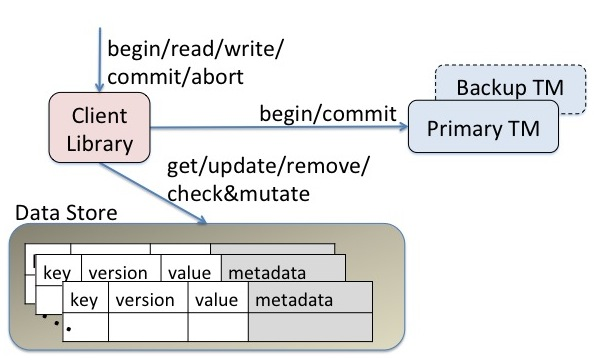
\includegraphics[width=0.48\textwidth]{FragolaComponents.jpg}
\caption{Transaction processing architecture: A client library exposes an  API for  executing transactions of data store operations. 
A centralized Transaction Manager handles transaction begin and commit requests, while data is written directly to the underlying data store.
The TM has a backup for high availability.}
\label{fig:components}
\end{figure}

\subsection{Data store}
\label{ssec:data-model}

The  data store holds  \emph{objects} (often referred to as \emph{rows}) identified by unique \emph{keys}.
Each row can consist of multiple \emph{fields}, representing different \emph{columns}. 
We consider multi-versioned objects, where object values are associated with \emph{version numbers}, and
multiple versions associated with the same key may co-exist in the data store.
\remove{
Thus, at any given time, an object holds a tuple \tuple{key,\tuple{version,value}+}, where value
can be structured to consist of multiple columns.
}
We further assume that a write operation can specify the version number it writes to.
%monotonically increasing ??
%\paragraph{API} 
The  data store provides the following API:
\begin{description}
\item [\code{get(key, version)}] --  Returns the requested version of the requested key.
%if no version is provided, returns the latest; 
%if no field is provided returns the entire record. 
%\item 
The API further allows traversing (reading) earlier versions of the same key in descending order.
\item [\code{update}(key, version, fields, values)] -- 
creates or updates an object, setting the specified fields to the specified values. 
If the version already exists, its value is updated; otherwise, a new version is added. 
\remove{The data store may buffer the write in memory until an ensuing flush. }
\item [\code{remove(key, version)}] -- removes an object with the given key and version.
\item [\code{check\&mutate}(key, version, field, old, new)] -- checks the record associated with key and version. 
If field holds old, replace it with new   and return true; otherwise return false.
\remove{ \item [\code{flush}] -- persists all previous updates to disk.}
%data stores often provide means to atomically read and update a single object, e.g., HBase exports check\&mutate operations, which are 
%internally implemented using a per-row RW lock.
%, whereas BigTable supports row transactions. 
%We will extend this capability below in order to implement certain atomic operations at the data store level.
\end{description}

A separate process performs garbage collection of obsolete versions.

\subsection{Transaction semantics} \label{ssec:transactions}

TPSs provide \emph{begin} and \emph{commit} APIs for delineating transactions: 
a \emph{transaction} the sequence of \emph{read} and \emph{write} operations on different objects 
that occur between begin and commit. Note that transactional reads and writes are implemented using the 
datastore's get and put operations.
Two transactions are said to be \emph{concurrent} if 
their executions overlap, i.e., one of them begins between the begin time and commit time of the other;
otherwise, we say that they are \emph{non-overlapping}.

A TPS  ensures the ACID properties for transactions:
\emph{atomicity} (all-or-nothing), \emph{consistency} (preserving each object's semantics), 
\emph{isolation} (in that concurrent transactions do not see each other's partial updates), and 
\emph{durability} (whereby updates survive crashes).

Different isolation levels can be considered for the third property. We consider a variant of 
snapshot isolation~\cite{DBLP:conf/sigmod/BerensonBGMOO95} that, similarly to \emph{generalized snapshot isolation}~\cite{DBLP:conf/srds/ElniketyZP05}, relaxes  the real-time order requirement. 
Nevertheless, our implementation only relaxes the ordering of fast path  transactions (described in Section~\ref{sec:alg}) 
relative to regular ones (that do not use the fast path); regular transactions continue to satisfy SI amongst themselves. 

Our correctness condition satisfies the key ``snapshot'' property of SI, which ensures that a transaction reading from the  database
does not see a mix old and new values. For example, if a task updates the values of two stocks, 
then no other transaction may observe the old value of one of these stocks and the new value of the other.
However, it relaxes the real-time order guarantee of SI by allowing (fast-path) transactions to take effect `in the past'.  
 \remove{ 
Similarly, a regular transaction overlapping
two fast path ones may observe an update of the second and miss an update by the first,  as illustrated in 
}
Figure~\ref{fig:ltx-rt}, shows an example where fast path transaction FP2 is ordered `in the past'.
%Yet we do enforce real-time order on regular transactions as well as on all updates of the same key.

\begin{figure}[ht]
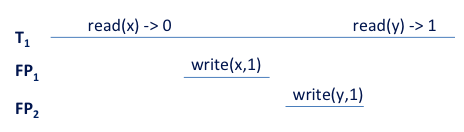
\includegraphics[width=\columnwidth]{figs/FP-semantics}
\caption{Possible violation of real-time order among fast path transactions. Regular transaction $T_1$
reads $x$ before it is updated by fast path transaction $FP_1$ and reads $y$ after it is updated by fast path transaction $FP_2$ even 
though $FP_2$ occurs after $FP_1$. 
%$T1$'s global version is $10$, and its skips the local version clocks of the regions holding $x$ and $y$ to $10$ when reading from them.
}
\label{fig:ltx-rt}
\end{figure}

Specifically, our correctness condition stipulates that
the system enforces a total order ${\cal T}$ on all committed transactions, so that
\begin{enumerate}
    \setlength{\itemsep}{0pt}
    \setlength{\parskip}{0pt}
    \setlength{\parsep}{2pt}  
%\item
%regular transactions (though not FP ones) are ordered in ${\cal T}$  according to their commit times;
\item
non-overlapping transactions 
%(regular and FP) 
that update the same key occur in ${\cal T}$  in order of their commit times;
\item
each  transaction's read operations see a consistent snapshot of the database reflecting 
a prefix of  ${\cal T}$; 
%and  
%that includes at least all regular transactions committed prior to its start time; and 
\item
 a transaction commits only if none of the items it updates is modified by a transaction ordered in ${\cal T}$ after
 its snapshot time and before its commit time.
 \end{enumerate}

\remove{ % OLD SI definition - no relaxation of RTO
More precisely, 
SI enforces a total order on committed transactions according to their commit times so that 
\begin{enumerate}
    \setlength{\itemsep}{0pt}
    \setlength{\parskip}{0pt}
    \setlength{\parsep}{2pt}  
\item
each transaction's read operations see a consistent snapshot of the database reflecting write operations by
 exactly those transactions that committed prior to the transaction's start time; and 
\item
 a transaction commits only if none of the items it updates has been modified since that snapshot.
 \end{enumerate}
 } %Remove
 
Note that as with SI, two concurrent transactions conflict only if they both \emph{update} the same item.  
In contrast, under serializability, a transaction that updates an item also conflicts with transactions that \emph{read} that item. 
Snapshot isolation is thus amenable to implementations (using multi-versioning) that 
allow more concurrency than serializable ones, and hence scale better.
It is therefore provided by popular database technologies such as Oracle, PostgreSQL, and SQL Server,
and TPSs such as Percolator, Omid, Tephra, and  CockroachDB.

Following a commit call, the transaction may successfully \emph{commit}, whereby all of its operations take effect;
in case of conflicts, (i.e., when two concurrent transactions attempt to update the same item), the transaction may
\emph{abort}, in which case none of its changes take effect. 



%An abort may also be initiated by the programmer, e.g., 
%on encountering an error. Applications typically retry a transaction upon  abort. 


%%%The data is \emph{partitioned} (or sharded), and each object belongs to one region. 
%%%%Global transactions may span multiple regions, and atomically commit or abort on all. 
%%%\emph{Local transactions} are ones that access a single region.


\section{Low-latency Transactions with \sys} \label{sec:ll}


We now describe \sys, a scalable low-latency TPS.
% on top of HBase. 
\sys\ is an evolution of the open-source Omid TPS, redesigned to reduce latency.
We begin in Section~\ref{ssec:schema} with some background on the modus operandi of existing TPSs that support SI, including Omid. 
We will see that, while many TPSs follow a similar schema,  they make different design choices when implementing this schema. 
We discuss the design choices of \sys\ in Section~\ref{ssec:ll-txns}. 
We then proceed to give a detailed description of the \sys\ protocol
in Section~\ref{ssec:ll}.

\subsection{Background: Schema of TPS operation}
\label{ssec:schema}


In many TPSs, transaction processing follows the following general schema, outlined in Algorithm~\ref{alg:schema}, 
while systems vary in their implementations of each of the steps.

\remove{
For example, whereas most systems rely on a centralized service for timestamp allocation~\cite{OmidICDE2014,Omid2017,tephra,Percolator2010}, this is not essential~\cite{cockroach}; similarly, validation (conflict detection) can use a centralized service~\cite{OmidICDE2014,Omid2017,tephra}, per-transaction entries in a global table~\cite{cockroach}, or distributed locking and validation~\cite{Percolator2010}. 
Different ways to implement this schema are  discussed in Section~\ref{sec:context}.
We now overview the phases a transaction goes through, focusing on Omid's approach.
}

\begin{algorithm}[tb]
\begin{algorithmic}[1]
\small
\Procedure{begin}{}
\State obtain read timestamp $ts_r$ 
\EndProcedure
\Statex

\Procedure{write}{key, value} \Comment transactional write
\State optionally check for conflicts and abort if found 
\State indicate write intent for key with value and $ts_r$
\State add key to local write-set
\EndProcedure
\Statex

\Procedure{read}{key} \Comment transactional read
\If{key has write intent}
	\State resolve, possibly abort writing transaction \label{l:resolve}
\EndIf
\State return highest version   $\le ts_r$ of key
\EndProcedure

\Statex

\Procedure{commit}{write-set, $ts_r$}
\Statex \Comment check for write-write conflicts  \label{l:validate}
\If{validate(write-set, $ts_r$)}  
	\State obtain commit timestamp $ts_c$
	\State \Comment commit all write intents with version $ts_c$
	\State atomically and persistently indicate commit   \label{l:commit}
\Else
	\State abort	
\EndIf
\State post-commit: update meta-data
\EndProcedure

\end{algorithmic}
\caption{TPS operation schema.} 
\label{alg:schema}
\end{algorithm} 


\paragraph{Begin.} 
  When a transaction begins, it obtains a read timestamp (version) $ts_r$ for reading its consistent snapshot.
  %, and unique transaction id.   The two can be combined (i.e., $ts_r$ can serve as the  transaction id, provided that it is unique).
 In most cases, this is done using a centralized \emph{transaction manager (TM)}~\cite{Percolator2010,OmidICDE2014,Omid2017,tephra},
 sometimes called timestamp oracle. 
%  In CockroachDB, the timestamp is based on a local clock that is ``close to'' real-time and preserves causality 
 % across regions, and unique transaction ids are used to break ties in case timestamps (from different regions) are identical. 

\paragraph{Transactional writes.} 
 During a transaction, a write operation indicates its \emph{intent} to write to a single object a certain new value with a certain version number.
%a dedicated \emph{commit} column in the object indicates that the write is tentative.
In Omid, the version is the transaction's $ts_r$, which exceeds all versions written by transactions that committed before the
current transaction began. Note that the version order among concurrent transactions that  attempt to update the same key is immaterial, 
since all but one of these transactions are doomed to abort. 

It is possible to buffer write intents locally in the course of the transaction, and add the write intents to the data store at commit time~\cite{Percolator2010}.

In some solutions writes check for conflicts before declaring their intents~\cite{cockroach}, whereas in others, 
all conflict detection is deferred to commit time~\cite{Percolator2010,OmidICDE2014,Omid2017,tephra}. 

\paragraph{Transactional reads.} 
The reads of a given transaction obtain a consistent snapshot of the data store at logical time (i.e., version) $ts_r$.
Each read operation retrieves the value of a single object associated with the highest timestamp that is 
smaller or equal to the transaction's $ts_r$. 

On encountering a write intent, read cannot proceed without determining whether the tentative write should be included in its snapshot,
for which it must know the writing transaction's commit status. 
To this end, TPSs keep per-transaction \emph{commit entries}, which are the source of truth regarding the transaction status 
(pending, committed, or aborted). 
This entry is updated in line~\ref{l:commit} of Algorithm~\ref{alg:schema} as we explain below, 
and is checked in order to resolve write intents in line~\ref{l:resolve}.
In some cases~\cite{Percolator2010,cockroach,Omid2017}, when the writing transaction status is undetermined, the read may forcefully abort
it by updating the commit entry accordingly.

%Similarly, the solution we implement in \sys\ forces the transaction with the pending write intent to abort. 

  \paragraph{Commit.} 
  Commit occurs in four steps:
  \begin{enumerate}
  \item
  Obtain a commit timestamp, $ts_c$. 
  In most cases, e.g.,~\cite{Percolator2010,OmidICDE2014,Omid2017,tephra}, 
  this is the value of some global clock maintained by a centralized entity. 
  \item \emph{Validate} that the transaction does not conflict with any concurrent transaction that has committed since it 
had begun.  For SI, we need to check for write-write conflicts only. 
If write intent indications are buffered, they are added at this point~\cite{Percolator2010}.
Validation can be centralized~\cite{OmidICDE2014,Omid2017,tephra} or distributed~\cite{Percolator2010,cockroach}. 


\item \emph{Commit} or abort in one  irrevocable atomic step. This is achieved by persistently writing to the \emph{commit entry}, 
  which can reside in a global table~\cite{Omid2017,cockroach} or alongside the first  key written by 
  the transaction~\cite{Percolator2010}.  
  
 \item \emph{Post-commit}: 
  Finally, a transaction changes its write intents to
  persistent writes in case of commit, and removes them in case of abort. This
  step is not essential for correctness, but reduces the overhead of future transactions. It
  occurs after the transaction is persistently committed or aborted via the commit entry, 
  and can be done asynchronously.
  %in
  %order to reduce the overhead of future transactions (by sparing them the need to check the commit entry)
  %and to garbage collect   obsolete information. 
 \end{enumerate}
 
  \remove{Note that whenever a transaction encounters a write
  indication in the collect phase it must access the commit entry in order to
  check the transaction's commit status. Once the post-commit phase is over, future
  transactions no longer incur this overhead for keys updated by the terminated
  transaction.}

\subsection{\sys\ design choices}
\label{ssec:ll-txns}

We now discuss our design choices, which are summarized and compared with other TPSs in  Table~\ref{table:design-space}. 

\begin{table*}[htb]
\small
\centerline{
\begin{tabular}{|l|ccccc|}
\hline
 & 
 \multicolumn{2}{c}{		 validation} & 
  \multicolumn{2}{c}{commit  entry}	& 
 resolving write intents\\
TPS	
& 	
scheme & time & 
location& update & 	
on read may cause abort	\\
\hline
Percolator 	& {\bf D} & commit & {\bf D} & {\bf D} & yes \\
Omid1, Tephra 	& {\bf C} & commit & {\bf R} & {\bf C} & no\\
Omid  		& {\bf C} & commit & {\bf C} & {\bf C} & no\\
CockroachDB	& {\bf D} & write     & {\bf C} & {\bf D} & yes\\
\sys			& {\bf C} & commit & {\bf D} & {\bf D} & yes\\
\hline
\end{tabular}
}
\caption{Design choices  in TPSs. {\bf C} -- centralized,  {\bf D} -- distributed, {\bf R} -- replicated.}
\label{table:design-space}
\end{table*}


\paragraph{Centralized validation.}

Percolator, the first TPS in this vein, used a distributed commit protocol that locked all written objects during validation. 
Unfortunately, while an object is locked, other transactions attempting to access it are blocked.
Since clients may stall or fail while holding a lock, Percolator detects failures of unresponsive 
clients and aborts transactions on their behalf. 
To eliminate the need for such failure detection and recovery, newer systems prefer to rely on 
a centralized TM for validation~\cite{OmidICDE2014,Omid2017,tephra}.


CockroachDB~\cite{cockroach}  takes a different approach: it performs distributed validation at write time, by replacing writes with atomic validate-and-write 
operations that can abort either the current transaction or a conflicting one. Since CockroachDB's approach slows down transactional writes 
while Omid's centralized conflict detection is extremely scalable~\cite{Omid2017},
%(capable of sustaining orders of magnitude higher throughput than the network~\cite{Omid2017}),  
\sys\ adopts the centralized validation mechanism from Omid. 


\paragraph{Distributed commit entry.}
The early generation of Omid~\cite{OmidICDE2014} (referred to as Omid1) and Tephra replicate commit entries 
of pending transactions among all active clients, 
which consumes high bandwidth and does not scale. Omid and CockroachDB instead use dedicated tables. CockroachDB updates the table in a distributed manner, 
while Omid has the centralized TM persist all commits. 
Our experiments show that the centralized access to commit entries is Omid's main scalability bottleneck, 
and while this bottleneck is mitigated via batching commit table updates, this also increases latency.
Omid chose this  option as it was designed for high throughput. Here, on the other hand, we target  low latency. 

We therefore opt to follow the design of Percolator, which stores each transaction's commit entry alongside its first written key,
which we call the \emph{leader}, and stores pointers to this leader at all other keys written by the transaction. 
Thus,  transaction entries can be updated in parallel by 
independent clients, and such updates are no longer a performance bottleneck. 
We will see below that this modification reduces latency
by up to an order of magnitude on small transactions.

\paragraph{Write intent resolution.}

As in other TPSs, reads resolve write intents via the commit entry.
If the transaction status is committed, the commit time is checked, and, if smaller than or equal to $ts_r$, it is taken into account;
if the transaction is aborted, the value is ignored.
In case the transaction status is pending, \sys, like Percolator and CockroachDB, has the reader
force the writing transaction to abort. This is done using an atomic check\&mutate operation to set the status in the
writing transaction's commit entry to aborted.

Omid and Tephra, on the other hand, do not need to force such aborts, because they ensure that  if the read sees a write intent
by an uncommitted transaction, the latter will not commit with an earlier timestamp than the read.
This is achieved by a single TM that allocates timestamps, performs validation, and writes the commit entry.
It either delays begin requests until all transactions that concurrently attempt to commit complete (as in Omid),
or sends information about all these transactions to the beginning client (as in Omid1 and Tephra).

\remove{

The centralized service, called Transactional Status Oracle (TSO), maintains an in-memory hash table mapping keys to 
commit timestamps ($ts_c$) of transactions that last wrote them. A conflict arises whenever a key in a transaction's write-set has been written 
with a timestamp higher than its $ts_r$. 
In case the conflict detection service crashes, all pending transactions are aborted, and it can be immediately restarted with an empty table, because only conflicts with concurrent transactions need to be checked. 


%
The possibility of reads aborting pending transactions means that commit attempts (line~\ref{l:commit}) have to  
check whether the transaction is aborted atomically with writing the commit status.


\subsection{Local transactions in \sys}
\label{ssec:fp-impl}
To support local transactions, we implemented the algorithms and APIs described in Section~\ref{sec:alg}. Each Hbase region server maintains an LVC which is updated whenever a transaction accesses it. Omid's API was extended to support FP transactions, and the write stage in regular transactions was modified to use checkAndMutate instead of put. 


 }
 
\begin{figure}[!t]
  \centering
  
  \begin{subfigure}[t]{\columnwidth}
      \centering
    \begin{tabular}{|c|c|c|c|c|}
      \hline
      key & value & version & commit& leader\\
      \hline
      \hline
      k1 & a & 3 & &\\
      \hline
      k2 & b & 3 & &k1\\
      \hline
      k2 & c & 3 & &k1\\
      \hline
    \end{tabular}
	\caption[]{Tentative transaction}
    \label{fig:model:tentative}
  \end{subfigure}
  
  \begin{subfigure}[t]{\columnwidth}
    \centering
    \begin{tabular}{|c|c|c|c|c|}
      \hline
      key & value & version & commit& leader\\
      \hline
      \hline
      k1 & a & 3 & 7&\\
      \hline
      k2 & b & 3 & &k1\\
      \hline
      k2 & c & 3 & &k1\\
      \hline
    \end{tabular}
	\caption[]{Committed transaction}
    \label{fig:model:committed}
  \end{subfigure}


  \begin{subfigure}[t]{\columnwidth}
    \centering
    \begin{tabular}{|c|c|c|c|c|}
      \hline
      key & value & version & commit& leader\\
      \hline
      \hline
      k1 & a & 3 & 7&\\
      \hline
      k2 & b & 3 & 7&\\
      \hline
      k2 & c & 3 & 7&\\
      \hline
    \end{tabular}
	\caption[]{Post-committed transaction}
    \label{fig:model:postcommit}
  \end{subfigure}

  
  \caption{Different stages of metadata during a transaction. The $txid$ the transaction received from the begin stage is 3, and the $ts_c$ it received when committing is 7. The leader chosen for this transaction is k1 }
  \label{fig:model}
\end{figure}


\begin{algorithm}[t]
  \begin{algorithmic}
    \begin{small}
      \Procedure{get(key)}{} 
      \For{rec $\leftarrow$ ds.get(\emph{key}, versions down from $ts_r$)}
      \If{rec.commit$\not=$nil} \Comment not tentative
      \If{rec.commit $< ts_r$}  \State return rec.value \EndIf
      \Else \Comment tentative
      \State value $\leftarrow$ {\sc GetTentativeValue(rec)}
      \If{value $\not=$nil}  
	  \State return value
      \EndIf
      \EndIf
      \EndFor
      \EndProcedure
      \Statex
      \Procedure{GetTentativeValue(rec)}{} 
      \State leader $\leftarrow$ rec.leader
      \State $tx_c$ $\leftarrow$ checkAndInvalidate(leader)
      \If{$tx_c$ $\not=$ nil} \Comment  committed
      \State update rec.commit \Comment helping 
      \If{$tx_c$ $< ts_r$}  return rec.value \EndIf
      \Else

      \State  return nil
      \EndIf
      \EndProcedure
    \end{small}
  \end{algorithmic}
  \caption{\sys's \emph{get(key)} operation.} 
  %for transaction with read timestamp $ts_r$.}
  \label{fig:get-pseudocode}
\end{algorithm} 



\Yoni{ explain here or in \ref{sec:ll-txns} that each key has multiple versions, we use $txd$ $tx_r$ $tx_c$....}

\subsection{Transaction metadata}
\label{ssec:tso}
\Yoni{make sure Idit defines  in section \ref{sec:ll-txns}}
Figure~\ref{fig:model} shows the metadata of a transaction during its stages of execution. For each version of a key in the data store we add 3 additional fields: (1) A \emph{version} field, which holds the $txid$ of the transaction that wrote it, in our implementation the $tx_r$ received at the begin stage is used as the $txid$. (2) A \emph{commit} field, which indicates whether the data is tentative or committed, if it's committed, the value will be the transaction's $ts_c$. (3) A \emph{leader} field. Since the transaction commit needs to be an atomic step, one key from the transaction's write set is chosen to be the \emph{leader} of that transaction, and when the transaction is committed a single atomic write is initiated to the \emph{leader's} commit field with the transaction's $ts_c$. Transaction read operations refer to the key's \emph{leader} to find out whether the value has been committed or not.




\subsection{Client-side operation}
\label{ssec:client}

\paragraph{Begin}
The client obtains from the TSO a read timestamp $ts_r$, which also becomes its transaction id ($txid$).


\paragraph{Get}
Algorithm~\ref{fig:get-pseudocode} describes \sys's implementation of Algorithm~\ref{alg:schema} READ procedure.
The data store's get operation is referred to as ds.get(key,version). The algorithm traverses records pertaining
to key with versions smaller than $ts_r$, latest to earliest, and returns the first key that is committed. Upon
encountering a tentative record (with commit=nil), the algorithm will get the leader's record from the data store,
read its $ts_c$ from the \emph{commit} field and return the key if the $ts_c$ is smaller than $ts_r$. To ensure SI,
if the leader's \emph{commit} field is nil, the transaction that leader represents must be aborted \Yoni{example here?}. The checkAndInvalidate function will atomically read the \emph{commit} field and if its value is nil, will insert an invalidation symbol in it. When a transaction commits, it atomically checks it hasn't been invalidated before inserting the $ts_c$ to the \emph{commit} field.

\paragraph{Put}
The client adds the tentative record \emph{(key, value, txid, nil,leader)} to the data store.
The leader is chosen to be the first key the client updates during a transaction.
To ensure monotonicity of written versions as seen in Section~\ref{ssec:regular-client-alg}, instead of using the standard \emph{put} operation the data store exposes, we must use checkAndMutate which will atomically put the record only if the latest version of the key is smaller than $ts_r$.


\paragraph{Commit}
The client requests \emph{commit(txid, write-set)} from the TSO. The TSO assigns it a commit timestamp $ts_c$ and checks for conflicts. If there are none, the client will write the $ts_c$ in the leader's \emph{commit} field. As explained at the Get stage, the transaction must atomically commit only if no other get invalidated it. This is done using the data store checkAndMutate function to read the invalidation symbol before writing the $ts_c$.
To avoid an extra RPC to the leader on every read, after a transaction is committed, a post-commit stage writes the $ts_c$ to the \emph{commit} field of every key in the write set of that transaction. 
Following a successful commit, the client adds $ts_c$ to all data items it wrote to.

\paragraph{Singleton Read}
\Yoni{This is the same as \ref{ssec:local-client-alg}}
\paragraph{Singleton Write}


\Yoni{what about WC and BRWC?}

\subsection{HBase region server}
\label{ssec:hbase}
\Yoni{is there something special to say here?}



%\section{High Availability} \label{sec:ha}
%\input{ha}


\section{Fast Path Transactions}
\label{sec:alg}

The goal of our fast path is to forgo the overhead associated with 
communicating with 
the TM to begin and commit transactions. This is particularly important for short transactions, where the begin and commit overhead is not amortized
across many operations.
We therefore focus on single-key transactions.

To this end, we introduce in Section~\ref{ssec:fast-api} a streamlined  \emph{fast path (FP)}
API that jointly executes multiple API calls of the original TPS.
We proceed, in Section~\ref{ssec:fast-algorithm}, to explain a high-level general fast path algorithm 
{for any system that follows the generic schema of  Algorithm~\ref{alg:schema} above}. 
Finally, in Section~\ref{ssec:fast-impl}, we describe our implementation of the fast path in \sys, and 
important practical optimizations we applied in this context.
 

\subsection{API and semantics}
\label{ssec:fast-api}

\paragraph{API.}
For brevity, we refer to the TPS's API calls  begin, read, write, and commit as \code{b, r, w}, and \code{c} respectively, and 
we combine them to allow fast processing.
The basic FP transactions are singletons, i.e., transactions that perform a single
read or write. These are supported by the APIs: 
\begin{description}
\item[brc(key)] -- begins an FP transaction, reads key within it, and commits.
\item[bwc(key,val)] -- begins an FP transaction,  writes val into a new version of key that exceeds all existing ones, and commits.
\end{description}

We further support a fast path transaction consisting of a read and a dependent write, via a pair of API calls:
\begin{description}
\item[br(key)] -- begins an FP transaction and  reads the latest version of key. 
Returns the read value along with a version ver.
\item[wc(ver, key,val)] -- 	validates that key has not been written since the  \code{br} call that returned ver, writes val into a new version of key, and commits.
\end{description}

Read-only transactions never abort, but \code{bwc} and \code{wc} may abort. 
If an FP transaction aborts, it can be retried either via the fast path again, or as a regular transaction.

We note that though the FP API richness can potentially complicate development, this drawback may be abstracted 
away by high-level access semantics. For example, a SQL implementation (e.g., Phoenix~\cite{Phoenix})
can select the most appropriate API in its query optimizer, transparently to the user.  


\remove{
A more elaborate example is a read-modify-write API: 
\begin{description}
\item[brwc(key,f)] -- begins an FP transaction,  reads the latest version of key, applies $f$ to it (on the server side), 
	writes the result into a new version of key that exceeds all existing ones, and commits.
\end{description}

To use the above API, the programmer has to encapsulate the transaction logic in a function for server-side processing. 
Alternatively, we allow FP transactions to unfold dynamically much like regular  transactions do.
A dynamic FP transaction may instead begin with a \code{br} call, perform client-side processing, and then call the following
function to update either the same or a different key: 

\begin{description}
\item[wc(key,val)] -- writes val into a new version of key that exceeds all existing ones, and commits.
\end{description}

Moreover, we do not restrict FP transactions to perform a single read -- any number of \code{r}'s may be called between the \code{br} 
and \code{wc}. The supported types of FP transactions are summarized in Table~\ref{table:fp-types}.
Note, however, that all calls must be directed at the same region, else the transaction is not local.
In case an FP transaction dynamically discovers that it needs to access additional regions, it is aborted and should be restarted as a regular transaction. 

\begin{table}[htb]
%\def\arraystretch{1.5}%  1 is the default, change whatever you need
\centerline{
\begin{tabular}{l  @{\hspace{2em}} l}
Call sequence & Transaction type\\
\hline
\code{br} & single read\\
\code{bwc} & single write\\
\code{br, r*} &  multi-read\\
\code{br, r*, wc} & multi-read, single write\\
\code{brwc} & server-side single-read-write\\
%\hline
\end{tabular}
}
\caption{Supported FP transaction types.}
\label{table:fp-types}
\end{table}

In principle, it would have been possible to also allow \code{w} calls in the span of an FP transaction, 
but in this case, it is not possible to forgo the two-phase execution. 
That is, the \code{w} calls would need to indicate write intents, and  to be atomically committed (or aborted) during the final \code{wc} 
(or \code{c}) call. 
Given the limited benefit and extra complexity of allowing many writes in FP transactions, we do not support this option in our solution.

}

\paragraph{Semantics.}
%\label{ssec:fast-semantics}

With FP transactions, 
\sys\ continues to establish a total order on all update transactions, both fast and regular ones, 
and transactions continue to observe snapshots that reflect a prefix of this total order.
However, we relax the real-time order guarantee of SI for FP transactions relative to regular ones. 
For example, an FP transaction may return 
an older value than the latest one committed by a regular transaction, essentially serializing the FP transaction `in the past'. 
Similarly, a regular transaction overlapping
two FP ones may observe an update of the second and miss an update by the first,  as illustrated in Figure~\ref{fig:ltx-rt},
where FP2 is ordered `in the past'.
Yet we do enforce real-time order on regular transactions as well as on all updates of the same key.

\begin{figure}[ht]
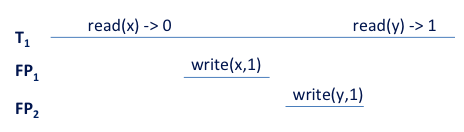
\includegraphics[width=\columnwidth]{figs/FP-semantics}
\caption{Possible violation of real-time order among fast path (FP) transactions. Regular transaction $T_1$
reads $x$ before it is updated by FP transaction $FP_1$ and reads $y$ after it is updated by FP transaction $FP_2$ even 
though $FP_2$ occurs after $FP_1$. 
%$T1$'s global version is $10$, and its skips the local version clocks of the regions holding $x$ and $y$ to $10$ when reading from them.
}
\label{fig:ltx-rt}
\end{figure}

Formally, the system enforces a total order ${\cal T}$ on all committed transactions, so that
\begin{enumerate}
    \setlength{\itemsep}{0pt}
    \setlength{\parskip}{0pt}
    \setlength{\parsep}{2pt}  
\item
regular transactions (though not FP ones) are ordered in ${\cal T}$  according to their commit times;
\item
non-overlapping transactions (regular and FP) that update the same key are ordered in ${\cal T}$  according to their commit times;
\item
each regular transaction's read operations see a consistent snapshot of the database reflecting 
a prefix of  ${\cal T}$ that includes at least all regular transactions committed prior to
its start time; and 
\item
 a transaction commits only if none of the items it updates is modified by a transaction ordered in ${\cal T}$ after
 its snapshot time ${\cal T}$.
 \end{enumerate}

Note that  ${\cal T}$  preserves causality because 
only transactions that  access different data objects can be re-ordered.


\subsection{Generic fast path algorithm}
\label{ssec:fast-algorithm}



\begin{algorithm}[htb]
\small
%\hspace{10mm}\\

\underline{Client-side logic:}
\begin{algorithmic}[1]
%\small
\Procedure{brc}{key} \label{l:brc}
\State rec  $\leftarrow$ ds.get(last committed record of key) 
\State  return rec.value
\EndProcedure
% \Statex
\Procedure{bwc}{key, value} 
%	\State old $\leftarrow$ ds.get(last version of key)
%	\If{old.commit = nil}  \Comment  tentative value -- abort 
%		\State return abort 
%	\EndIf
	\State return {ds.writeVersion}($\infty$, key, value)
\EndProcedure
% \Statex
\Procedure{br}{key} 
\State rec  $\leftarrow$ ds.get(last committed record of key) 
\State  return \tuple{rec.version, rec.value}
\EndProcedure
% \Statex
\Procedure{wc}{ver, key, value} 
\State return {ds.writeVersion}(ver, key, value)
\EndProcedure
\Statex
\algstore{fp}
\end{algorithmic}

\underline{Data store logic:}
\begin{algorithmic}[1]
\algrestore{fp}
%\small
\Procedure{writeVersion}{old, key, value} 
\Statex \Comment used by FP writes (\code{bwc} and \code{wc})
%\Atomic 
	\If{key has no tentative version $\wedge$\\
		\hspace{7mm} last committed version of key $\le$ old}
		\State ver $\leftarrow$ F\&I(key's maxVersion) $+1$   \label{l:fi}
		\State add \tuple{key, ver} with commit = ver  
		\State return commit
	\Else 
		\State return abort 
	\EndIf
%\EndAtomic
\EndProcedure
% \Statex
\Procedure{txRead}{$ts_r$, key}   \label{l:txr}
\Statex \Comment used by transactional read, once per key 
\State bump(key's maxVersion, $ts_r$)
\State return get(key)
\EndProcedure
% \Statex
\Procedure{txWrite}{$ts_r$, key}   \label{l:txw}
 \Statex \Comment used by transactional write
 \If{key has a committed version that exceeds $ts_r$} 
 	\State abort 
 \EndIf
 \State add \tuple{key, $ts_r$} with commit = nil  
\EndProcedure

\Procedure{txUpdate}{key, ver, $ts_c$}   \label{l:txu}
\Statex \Comment used by transactional post-commit 
\State bump(key's maxVersion, $ts_c$)
\State update commit field of \tuple{key, ver} to $ts_c$
\EndProcedure
\end{algorithmic}
\caption{Generic support for FP transactions; each data store operation is executed atomically.}
\label{alg:fp}
\end{algorithm}

The generic fast  path algorithm consists of two parts: 
client side-logic, and new atomic operations implemented in the  underlying data store.
It is presented in pseudocode in Algorithm~\ref{alg:fp}. 

Singleton reads (line~\ref{l:brc}) simply return the value associated with the  latest committed version of the requested key they encounter.  
They ignore tentative versions, which may lead to missing the latest commit in case its post-commit did not complete, 
but is allowed by our semantics. 
FP reads can forgo the begin call since they do not need to obtain a snapshot time a priori. 
They can also forgo the commit call, since they perform a single read, and hence their `snapshot' is trivially valid.

In case  \code{bwc} encounters a tentative version it does not try to resolve it, but rather simply aborts.
This may cause false aborts in case the transaction that wrote the tentative version has committed and did not 
complete post-commit, as well as in the case that it will eventually abort. 
In general, this mechanism prioritizes regular transactions over FP ones. We choose this approach since
the goal is to complete FP transactions quickly, and if an FP transaction cannot complete quickly, it might as well be 
retried as a regular one.
   
Such a singleton write has two additional concerns: (1) it needs to  produce a new version number that exceeds all committed ones and
is smaller than any commit timestamp that will be assigned to a regular transaction in the future.
(2)  It needs to make sure that conflicts with regular transactions are detected. 

We handle these concerns in a way similar to Mediator~\cite{mediator}.
Namely, we maintain the timestamps as two-component structures, consisting of a global version and a locally advancing sequence number.
In practice, we implement the two components in one long integer, with some number $\ell$ least significant bits
reserved for sequence numbers assigned by FP writes (in our implementation, $\ell=20$).
The most significant bits represent the global version set by the TM. The latter increases 
the global clock by $2^\ell$ upon every begin and commit request.

To support (1) a {\code{bwc}} transaction reads the object's latest committed version, and increments it. 
%This is different from~\cite{mediator} which aggregates multiple timestamps in a local clock and more like~\cite{cockroach} which reads and manipulates versions at the object's level.
The increment is done provided that it does not overflow the sequence number. 
In the rare case when the lower $\ell$ bits are all ones, the global clock must be incremented, and so the FP transaction aborts and is retried as a regular one. 

It is important to note that the singleton write needs to \emph{atomically} find the latest version and produce a new one that exceeds it, 
to make sure that no other transaction creates a newer version in the interim. This is done by a new \emph{writeVersion} function implemented 
at the data store level. In Section~\ref{ssec:fast-impl}
below, we explain how we implement such atomic conditional updates in HBase as part of \sys. 
The first parameter to writeVersion is an upper bound on the key's current committed version; since a singleton write
imposes no constraints on the object's current version, its upper bound is $\infty$.

Next, we address (2) -- conflicts between FP and regular transactions.
(Note that the atomic conditional write in \code{bwc} takes care of conflicts among singletons.)
In case an ongoing regular transaction writes to a key before \code{bwc} accesses it, 
\code{bwc} finds the tentative write and aborts. 

It therefore remains to consider the case that
a regular transaction $T_1$ writes to some key after FP transaction $FP_1$, but $T_1$ must abort because
%the key is updated between its snapshot time and update time. 
it reads the old version of the key before $FP_1$'s update. This scenario is illustrated in Figure~\ref{fig:why-bump}. 
Note that in this scenario it is not possible to move $FP_1$ to `the past' because of the read.

\begin{figure}[htb]
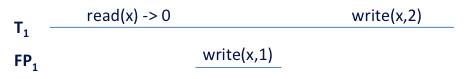
\includegraphics[width=\columnwidth]{figs/FP-why-bump}
\caption{Conflict between FP transaction $FP_1$ and regular transaction $T_1$.}
\label{fig:why-bump}
\end{figure}

In order for $T_1$ to detect this 
conflict, the version written by $FP_1$ has to exceed $T_1$'s snapshot time, i.e., $ts_r$.
To this end, we maintain a new field \emph{maxVersion} for each key, which is at least as 
high as the key's latest committed version. 
The data store needs to support two atomic operations for updating {maxVersion}.
The first is \emph{fetch-and-increment, F\&I}, which increments {maxVersion} and returns its
old value; F\&I throws an abort exception in case of wrap-around of the 
sequence number part  of  the version. 
The second operation, \emph{bump}, takes a new version  as a parameter and
sets  {maxVersion} to the maximum between this parameter and its old value.

Singleton writes  increment the version using F\&I  (line~\ref{l:fi}), and  
the post-commit of transactional writes  (line~\ref{l:txu}) bumps it 
to reflect the highest committed version.
In addition, every transactional read bumps the key's {maxVersion}
to the reading transaction's $ts_r$  (line~\ref{l:txr}), and
transactional writes (line~\ref{l:txw}) are modified to check for conflicts, namely, 
new committed versions exceeding their $ts_r$.

In the example of Figure~\ref{fig:why-bump}, $T_1$'s read bumps $x$'s {maxVersion} to its $ts_r$, 
and so $FP_1$, which increments $x$'s maxVersion, writes $1$ with a version that exceeds $ts_r$.
Thus, $T_1$'s write  detects the conflict on $x$. 

 Note that this modification of transactional writes incurs an extra cost on
 regular (non-FP) transactions, which we quantify empirically in Section~\ref{sec:eval}.  

The \code{br} and \code{wc} operations are  similar to \code{brc} and \code{bwc}, 
respectively, except that \code{wc} uses the version read by \code{br} as its upper bound
in order to detect conflicting writes that occur between its two calls.

\subsection{Implementation and optimization}
\label{ssec:fast-impl}

Associating a maxVersion field with each key is wasteful,
both in terms of space, and in terms of the number of updates this field undergoes.
Instead, when implementing support for \sys's fast path in HBase, we aggregate the maxVersions of many keys in a single variable, 
which we call the \emph{Local Version Clock (LVC)}; (similar local clocks were previously used in Mediator~\cite{mediator}
and CockroachDB~\cite{cockroach}).

Like many state-of-the-art data stores, HBase data is \emph{sharded} (partitioned) 
across many \emph{regions}, and is deployed on multiple  \emph{region servers}, each of which serves
several hundreds of regions. Our solution implements one LVC in each region server. 
Using a shared LVC reduces the number of updates:  
a transactional read modifies the LVC only if its $ts_r$ exceeds it. In particular, 
a transaction with multiple reads in the same region server needs to bump it only once. 

We implement the two required atomic methods - F\&I and bump on the LVC using atomic hardware operations (F\&I and CAS, respectively). 
In addition, 
HBase   natively supports  a check\&mutate operation, which holds a lock on the affected key for the duration of the operation.
Our implementation of the singleton write uses  check\&mutate to implement the atomic block, and calls the LVC's F\&I method inside this block.
Transactional reads and post-commits call bump from inside a check\&mutate  block where they perform their read and version update, respectively. 

Note that although check\&mutate only holds a lock on the affected key, the joint update of the key and the LVC is consistent
because it uses a form of two-phase locking: when check\&mutate begins, its locks the key, then the atomic access to the LVC
effectively locks the LVC during its update; this is followed by an update of the key's record and the key's lock being released.

The LVC is kept in memory, and is not persisted. Migration of region control across region servers, which HBase performs 
to balance load and handle server crashes, must be handled by the LVC management. 
In both cases, we need to ensure that the monotonicity of the LVC associated with the %(migrated or recovered) 
region is preserved. To this end, when a region is started in a new server (following migration or recovery), 
we force the first operation accessing it
in the new server to accesses the TM to increment the global clock, and then 
bumps the local clock to the value of the global clock.
Since the LVC value can never exceed the global clock's value, this bootstrapping procedure maintains its monotonicity.





\section{Evaluation} \label{sec:eval}


We describe our methodology and experiment setup in Section~\ref{ssec:methodology}, and present our results 
in Section~\ref{ssec:results}.

\subsection{Methodology}
\label{ssec:methodology}

\paragraph{Evaluated systems.}

We compare \sys\  to  state-of-the art TPSs and separately evaluate the effectiveness of its FP mechanism.
To this end, we compare four TPSs, all of which use HBase as the underlying data store -- Omid, \sysll, 
\syspc, and \sys. \syspc\ defers writes to commit time (as Percolator does), whence it writes and validates
keys using check\&mutate.
\remove{
\begin{description}
\item[\sys] -- the algorithm described in Section~\ref{sec:ll}, without support for FP transactions.
\item[\sys] -- single-key transactions use the FP API, 
whereas longer transactions use the standard API, 
and their transactional reads and writes are modified to access the LVC along with the data as described in Section~\ref{sec:alg}.
\item[Omid] -- the Apache Incubator version of Omid, on which we base our implementation of \sys. 
\item[2PC] -- an implementation (in the \sys\ framework) of Percolator's concurrency control mechanism:
Begins and commits use the TM only for timestamp allocation and not for conflict detection; conflicts are detected via 
\emph{Two Phase Commit (2PC)}.
\end{description}
}
In \sys, single-key transactions use the FP API, whereas longer transactions use the standard API. 
The other systems use the standard API only.

Note that both CockroachDB and Percolator use 2PC-based conflict resolution, so our \syspc\ mimics
their protocols. 
Direct comparison with the actual systems is not feasible because Percolator is proprietary and 
CockroachDB supports SQL transactions over a multi-tier
architecture using various components that are incompatible with HBase. 
We also do no compare \sys\ to Omid1 (and the similarly-designed Tephra), since Omid significantly
outperforms Omid1~\cite{Omid2017}.

To reduce latency, we configure the TPSs to perform the post-commit phase asynchronously, 
by a separate thread, after the transaction completes.

\remove{
In Omid and Vanilla \sys, all transactions use the standard API, namely 
delineating transactions with begin and commit calls.
In FP \sys, transactions that can use the FP API (specifically, singleton reads, singleton writes, 
and single-key read-writes) do so, whereas other transactions use the standard API.
}

\paragraph{Experiment setup.}

Our experiment testbed consists of nine 12-core Intel Xeon 5 machines with 46GB RAM and 4TB 
SSD storage, interconnected by 10G Ethernet. We allocate three of these to HBase nodes, 
one to the TM, one to emulate the client whose performance we measure, and four more to simulate 
background traffic as explained below. Each HBase node runs both an HBase region server and 
the underlying Hadoop File System (HDFS) server within 8GB JVM containers. 

Note that the only scalability bottleneck in the tested systems is the centralized TM.
HBase, on the other hand, can scale horizontally across thousands of nodes, each of which processes a small fraction of the total load. 
Since each node typically serves millions of  keys, data access rates remain load-balanced across nodes 
even when access to individual keys is highly skewed.  And since read/write requests are processed independently by each HBase node, 
their performance remains constant as the workload and  system size are scaled by the same factor. 

Thus, to understand the system's performance at scale, 
we can run transactions over a small HBase cluster with an appropriately-scaled load, 
but need to stress the TM as a bigger deployment would. 
We do this at a ratio of 3:1000; that is, we run transactions on a $3$-node HBase cluster and 
load the TM with a begin/commit request rate that would arise in a $1000$-node HBase cluster with the same per-node load.
For example, to test the client's latency at $100$K tps, we have the TM handle $100$K tps, and have  an HBase deployment of
three nodes handle read/write requests of $300$ tps. As explained above, 
the HBase latency at $100$K tps with $1000$ servers would be roughly the same as in this deployment.

We use four machines to generate the background load on the TM using a custom tool~\cite{Omid2017} 
that asynchronously posts begin and commit requests on the wire and collects the TM's responses. 
We note that although in this experiment the TM maintains a small number of client connections (serving many requests per connection), 
the number in a true $1000$-node system still falls well within the OS limit, hence no real bottleneck is ignored. 

We measure the end-to-end client-incurred latency on a single client node that generates transactions over the $3$-server HBase cluster. 
Note that the client also generates begin/commit requests, which account for \mbox{$\sim0.3\%$} of the TM's load.
The client runs the popular YCSB benchmark~\cite{Cooper:2010:BCS:1807128.1807152}, 
exercising the synchronous transaction processing API in a varying number of threads. 

\paragraph{Workload.}

Our test cluster stores approximately 23M keys ($\sim\!\!7$M keys per node). 
The values are 2K big, yielding roughly 46GB of actual data, replicated three-way in HDFS. The keys are hash-partitioned
across the servers. The data accesses are 50\% reads and 
50\% writes. The key access frequencies follow a Zipf distribution, generated following 
the description in~\cite{Gray:1994:QGB:191839.191886}, with $\theta=0.8$, which we derive from production 
workloads. \inred{In this distribution, the first key is accessed 3.5\% of the  time.}
%in Yahoo's deployment of Omid~\cite{Omid2017}. 
%Note that under this access distribution, data requests are load-balanced across nodes.

\noindent
We test the system with two transaction mixes:
\begin{description}
\item[Random mix] -- 
transaction sizes (number of reads and writes) follow a Zipf distribution with $\theta=0.99$, with a cutoff at $10$. 
With these parameters, $63\%$ of the transactions access three keys or less, and only $3\%$ access $10$ keys. 
We vary the system load from 30K to 500K transactions per second (tps). 
\item[BRWC] -- $80\%$ of the transactions are drawn from the random mix distribution, and $20\%$ perform a read
and then a write to the same key. 
\end{description}

We add the BRWC workload since single-key read+write transactions are common in production, but are highly unlikely to 
occur in our random mix, which uses random key selection with billions of keys.

\begin{figure}[htb]
	\centering
      	\includegraphics[width=0.48\textwidth]{figs/throughputlatency1.pdf}
	    \caption{Throughput vs.\ latency, transaction size = 1.}
        \label{fig:tl-1}      
\end{figure}


\begin{figure*}[hbt]
\centering
\begin{tabular}{ccc}
      \begin{subfigure}[t]{0.48\textwidth}
         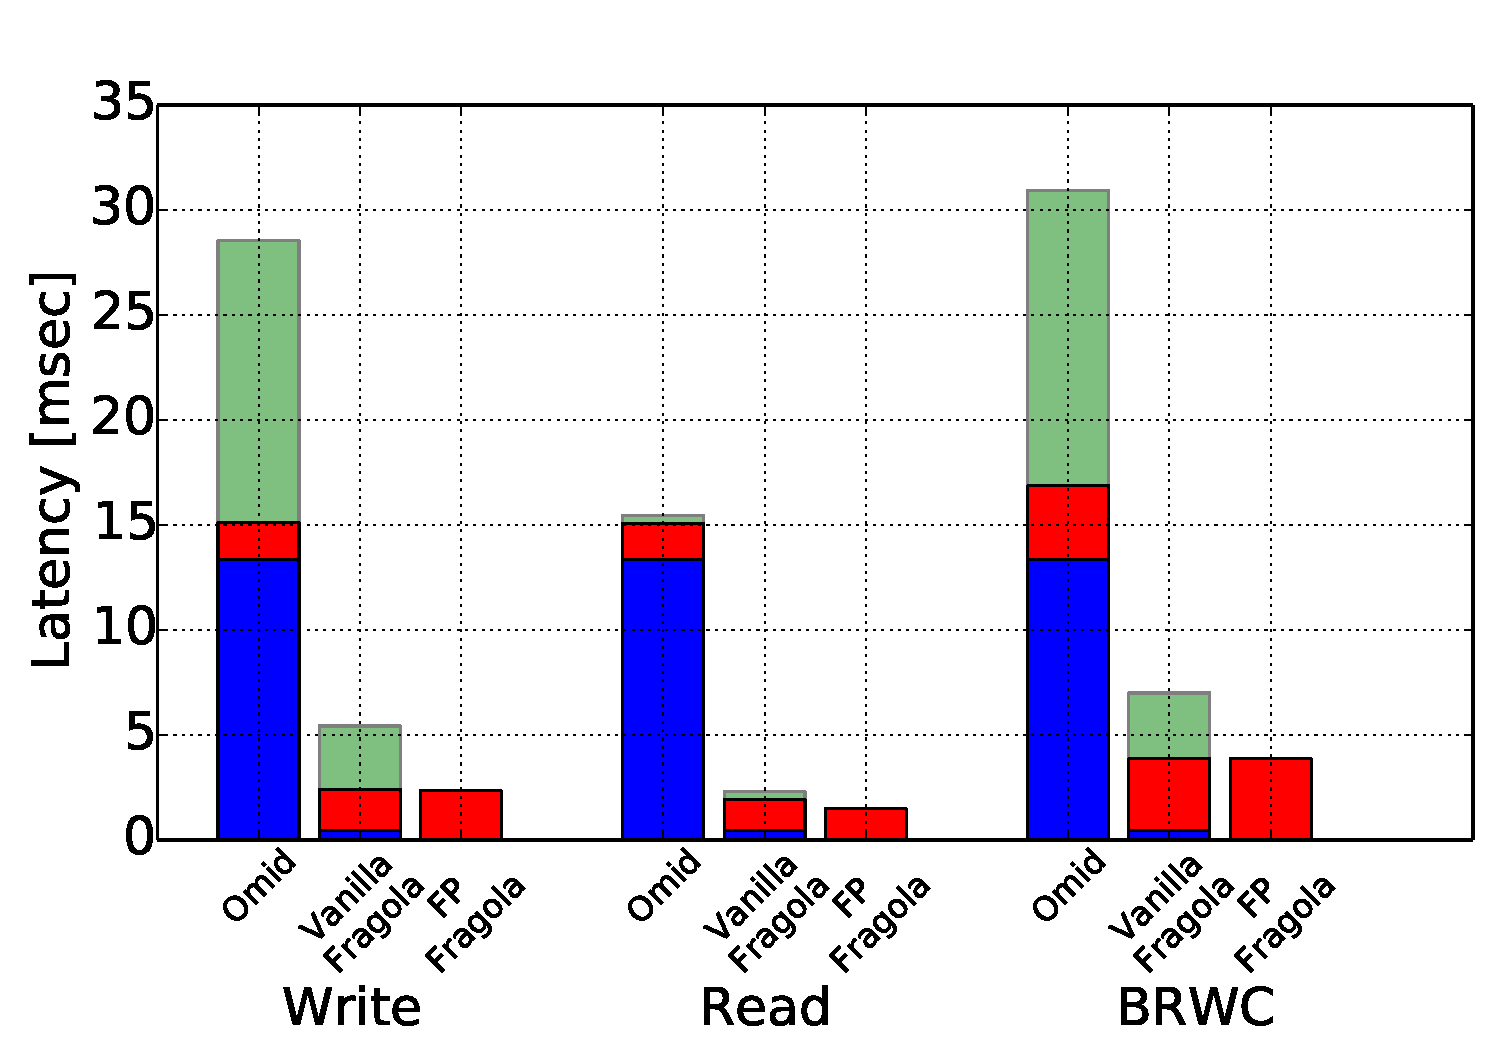
\includegraphics[width=\textwidth]{figs/latency_allPUTGET.pdf}
        \caption[]{Low load (100K tps).}
        \label{fig:stack-brc}

      \end{subfigure} 
    
& 
      \begin{subfigure}[t]{0.48\textwidth}
      	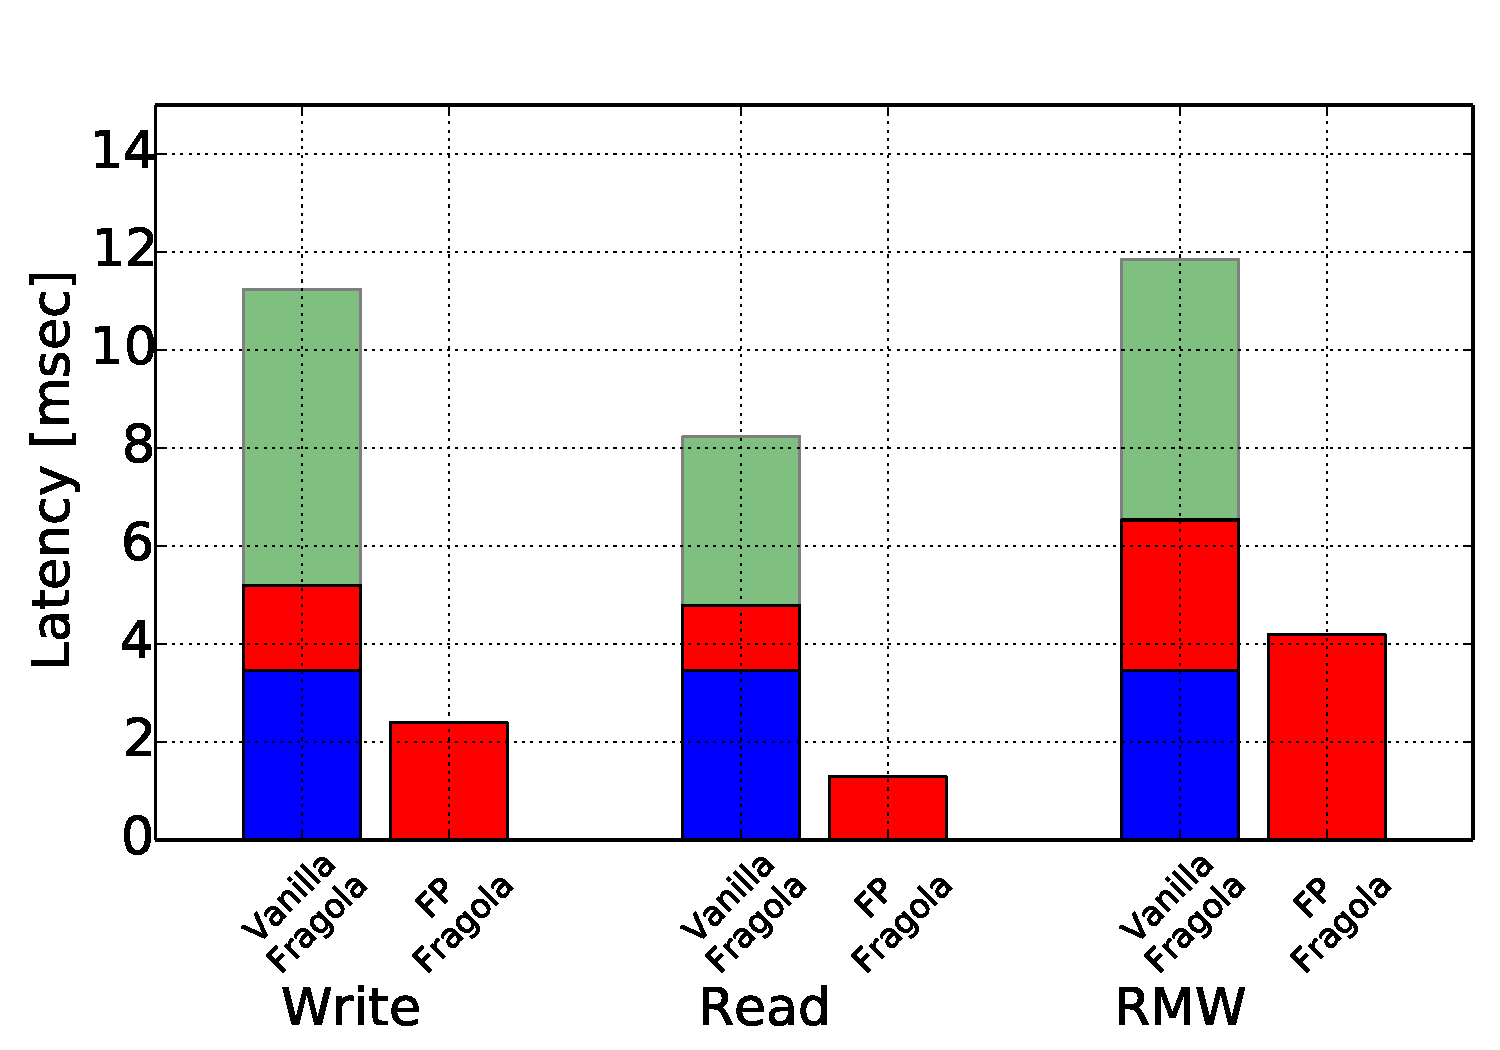
\includegraphics[width=\textwidth]{figs/latencyHighThrough_PUTGETRMW.pdf}
	\caption{High load (500K tps).}
	\label{fig:hightx}
      \end{subfigure}  & 

\end{tabular}
       \caption{Latency breakdown  for single-key transactions under  random mix workload. }
\end{figure*}


\subsection{Results}
\label{ssec:results}

\mypara{Throughput and latency of short transactions.} 
%
Recall that \sys\ is motivated by the prevalence of short transactions in production, and is designed with
the goal of accelerating such transactions.
Its advantage is less pronounced for long transactions, where the cost of begin and commit is amortized
across many reads and writes.
To make the comparison meaningful, we classify transactions by their lengths and whether they
access a single key, and study each transaction class separately. 

We begin with short transactions. 
Figure~\ref{fig:tl-1} presents the average latency of single-key transactions run as part of the random mix,
as a function of {system} throughput.
Figure~\ref{fig:stack-brc}  then zooms in on the latency of such transactions under 
a throughput of 100K tps, and breaks up the different factors contributing to it. 
Figure~\ref{fig:hightx}  presents a similar breakdown under a high load of 500K tps; Omid 
is not included since it does not sustain such high throughput.

As we can see, under light load, \sysll\ and \syspc\ improve the latency of Omid by 4x to 5x.
%, even without the fast path.
This is because in Omid, both begin and commit wait for preceding transactions to complete the writes of 
their commit entries; this stems from Omid's design choice to avoid the need for resolving pending write intents
by aborting transactions; see penultimate column in Table~\ref{table:design-space}. 
Single-key writes suffer from both the begin and commit latencies, whereas single-key reads  
suffer only from begins (Figure~\ref{fig:stack-brc}). \syspc\ has longer commit latencies and shorter write latencies
because it defers writes to commit time.

As load increases, Omid suffers from a well-pronounced bottleneck, and its latency at 250K tps is doubled, where the other systems
are unaffected. The extra delay in Omid is due to batching of commit record updates, 
which its TM applies to handle congestion~\cite{Omid2017}. 

Under low load, \sysll\ is slightly faster than \syspc\ (due to the latter's use of atomic check\&mutate). 
But under high load, \syspc\ is slightly better ($10\%$ faster on average for single-key transactions)   
due to the centralized conflict analysis becoming a bottleneck in \sysll.

The FP API delivers better performance for this traffic. For instance, under low load (Figure~\ref{fig:stack-brc}),
single writes take an average of 2.4ms using 
the {\code bwc} API versus 5.7ms in \sysll\ (and 5.9ms in \syspc). 
For comparison, a native HBase write takes roughly 2ms under this load.
A single read executed using {\code brc} takes 1.5ms, which is the average latency of a native HBase read,
versus 2.5ms as a regular transaction in \sysll\ (2.7ms in \syspc). 
For transactions that read and write a single key as part of the BRWC workload, 
%Their latency breakdown under a 100K tps throughput is shown in Figure~\ref{fig:rmw}.
the fast path implementation (consisting of \code{br} and \code{wc} calls) completes within 4ms,
versus 6.5ms for  \sysll, 7.1ms for \syspc, and 37.6ms for Omid. 
%
Under high load (Figure~\ref{fig:hightx}), the fast path is even more beneficial: it reduces the latency of 
both read and write by more than a factor of 2. 
%2.7, from 6.9ms  to 2.6ms, and the read latency by a factor of 2.2, from  3.7ms to 1.7ms.
%, read, and brwc from 11.24ms, 8.24ms, and 11.85ms to 2.4ms, 1.29ms, and 4.19ms respectively. 



\mypara{Long transactions.} 
We now examine longer transactions run as part of the random mix.
Figure~\ref{fig:throughput-latency} shows the results for transactions of lengths $5$ and $10$.
We see that the absolute latency gap of the new systems over Omid remains similar, but is amortized 
by other operations. Omid's control requests (begin and commit) continue to 
dominate the delay, and comprise $68\%$ of the latency of 10-access transactions (under low load).
In contrast, the transaction latency of \sysll\ (and \sys) is dominated by data access, 
as only $13\%$ (resp.~$18\%$)  of the time is spent on the control path. 
\syspc\ spends $66\%$ time executing commit  because it defers writes to commit time,
but this is offset by a shorter read/write execution time.

\begin{figure*}[t]
\centering{
\begin{tabular}{cc}

    \begin{subfigure}[t]{0.48\textwidth}
	\includegraphics[width=\textwidth]{figs/throughputlatency10.pdf}
	\caption[]{Throughput versus latency, transaction size = 10}
    \label{fig:tl-10}
  \end{subfigure} & 


  \begin{subfigure}[t]{0.48\textwidth}
	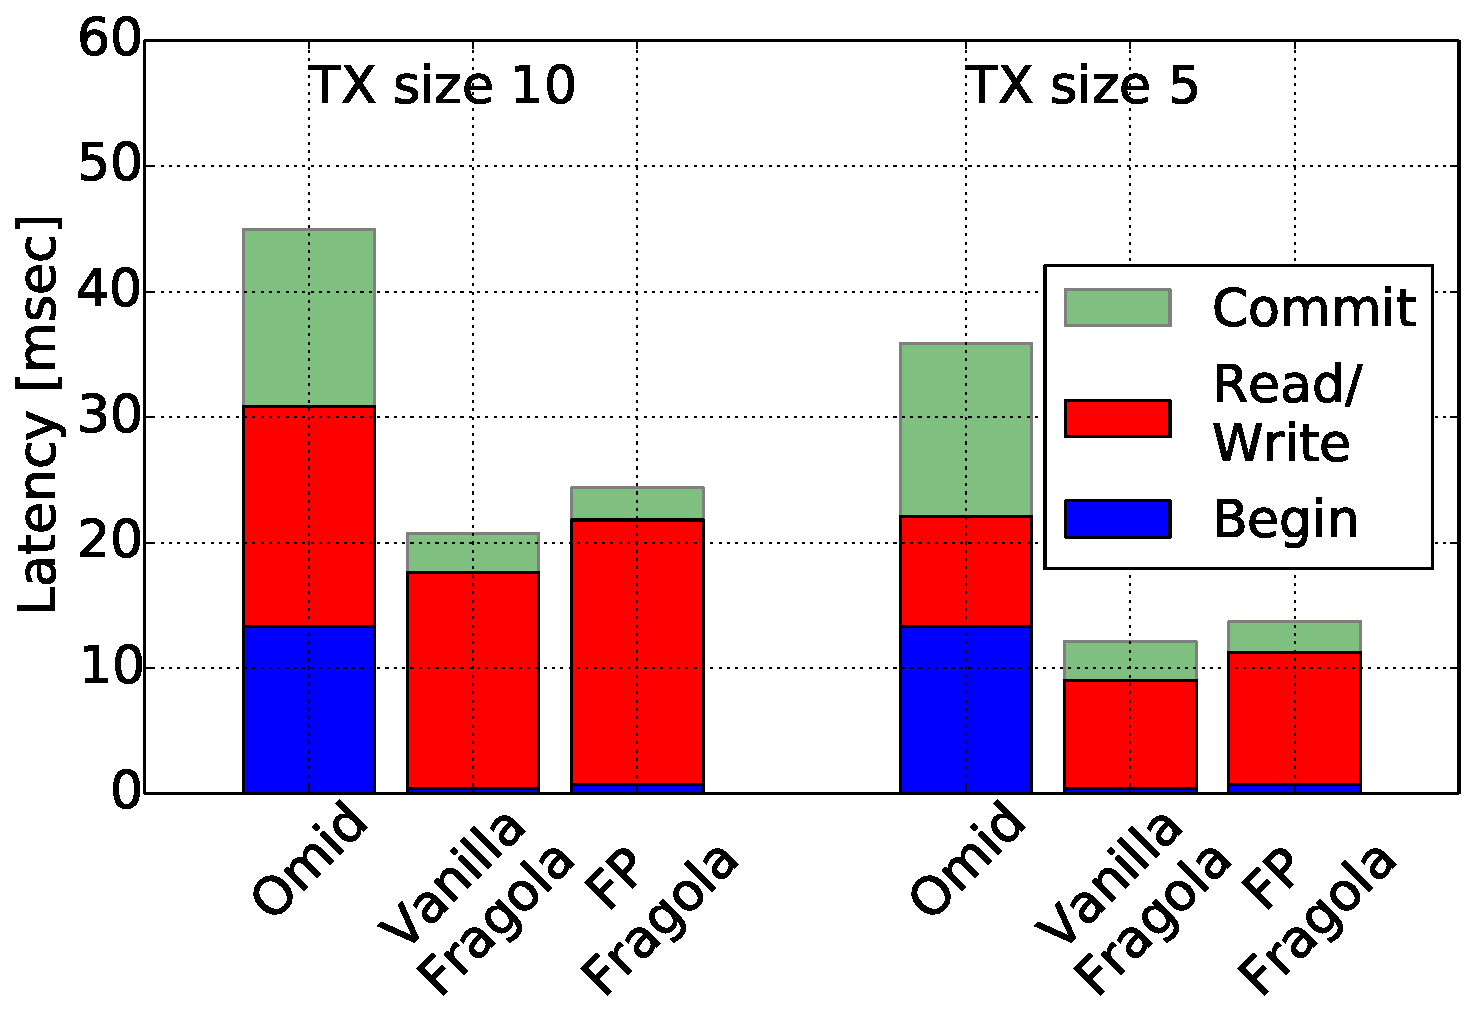
\includegraphics[width=\textwidth]{figs/latency_5_10.pdf}
	\caption[]{Latency breakdown, transaction size = 5, 10}
    \label{fig:stack-tx10}
  \end{subfigure} 
\end{tabular}  	
}		
  \caption{Latency vs.\ throughput  and latency breakdown  for long transactions in random mix workload. }
  \label{fig:throughput-latency}
\end{figure*}



The FP mechanism takes a toll on the data path, which uses atomic check\&mutate operations 
instead of simple writes. This is exacerbated for long transactions.
For example, a 10-access transaction takes 24.8ms with \sys, 
versus 21.7ms with  \sysll. The performance of \syspc\ with long transactions is similar to that of \sys\ -- e.g., 25.6ms for 10-access transactions -- 
because it also uses check\&mutate operations during the commit validation phase.

 

\begin{figure}[h!]
\centering
\begin{subfigure}[t]{0.48\textwidth}
\centerline{
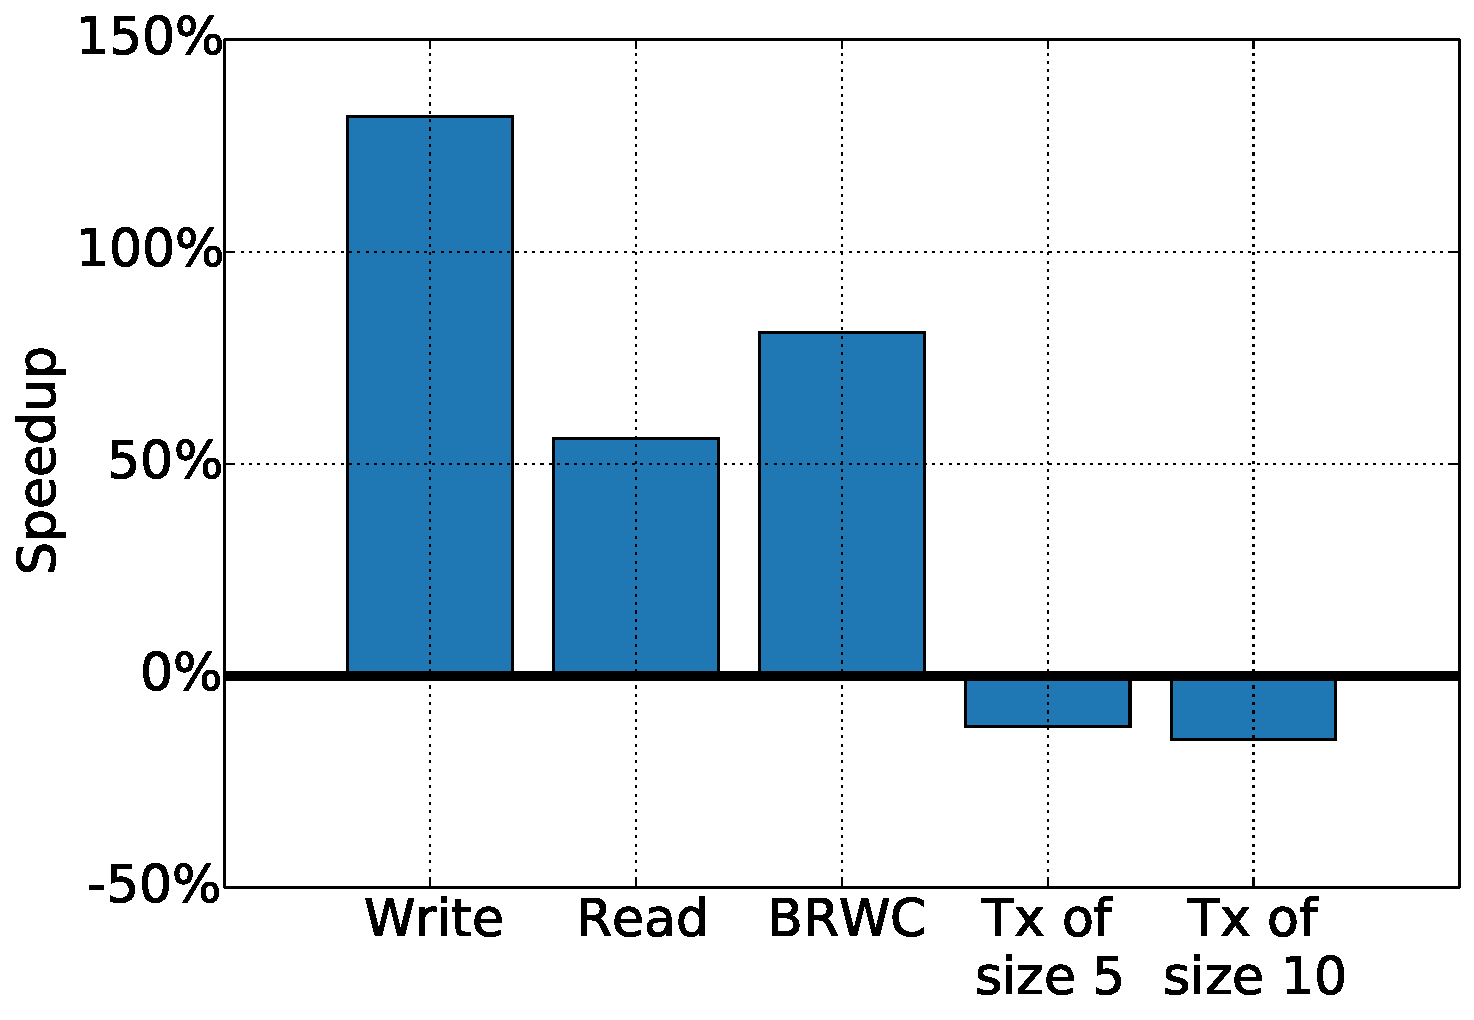
\includegraphics[width=.9\textwidth]{figs/low_speedup.pdf}
}
\caption{Low load (100 tps)} 
\label{fig:slowdown-low}
\end{subfigure} 
\begin{subfigure}[t]{0.48\textwidth}
\centerline{
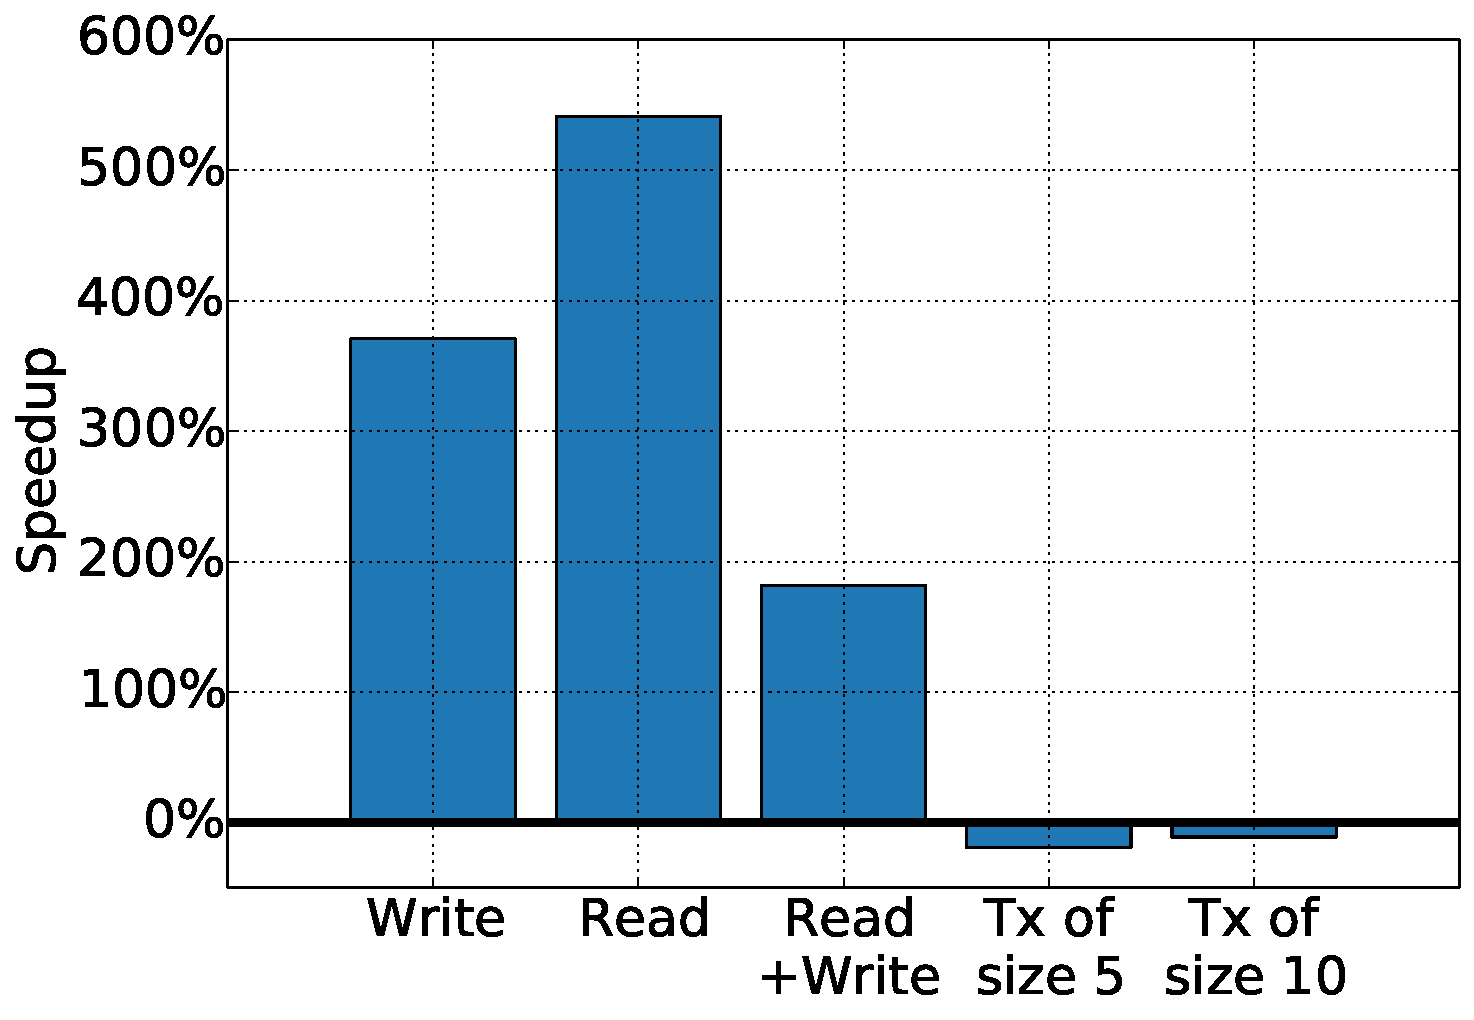
\includegraphics[width=.9\textwidth]{figs/high_speedup.pdf}
}
\caption{High load (500 tps)} 
\label{fig:slowdown-high}
\end{subfigure} 
\caption{Latency speedup with  fast path API in {\sys}.}
\label{fig:fp-tradeoff}
\end{figure}



Figure~\ref{fig:fp-tradeoff} summarizes the tradeoffs entailed by \sys\ relative to \sysll\ for the different transaction classes. 
We see that under low load (Figure~\ref{fig:slowdown-low}),
the speedup for single-write transactions is $2.3$x, whereas the worst slowdown is $13\%$. 
In systems geared towards real-time processing, this is a reasonable tradeoff, since long transactions 
are infrequent and less sensitive to extra delay.
Under high load (Figure~\ref{fig:slowdown-high}), the fast path is even more advantageous: the speedup for writes is $2.7$x.
%In systems geared towards real-time processing, this is a reasonable tradeoff, since long transactions 
%are infrequent and less sensitive to extra delay. Under the studied workload, e.g.,   FP \sys\/ is more desirable. 



\mypara{Abort rates.}

%Abort rates are extremely low -- between  $0.01\%$ and  $0.02\%$ -- for all systems. To Do: try a sharper Zipf.}  
We note that \sys\ yields slightly higher rates of transaction aborts compared to Omid 
(recall that \sysll\ aborts tentative writes in favor of concurrent reads, whereas  \sys\ also aborts
singleton writes in presence of concurrent tentative writes). However, the abort rates exhibited by all  
the systems are minor. 
Here, under the highest contention,  \sys\ aborts approximately \inred{$0.1\%$ }
of the transactions versus  \sysll's \inred{$0.08\%$ },   
 \syspc's \inred{XXX} 
and Omid's $0.07\%$ 
(the latter  is in line with production abort rates reported in Omid~\cite{Omid2017}).  




\section{Related Work} \label{sec:related}


The past few years have seen a growing interest in distributed 
transaction management~\cite{PattersonENAA12,Cowling2012,Aguilera2015,Balakrishnan2013,Thomson2012,eyal2013ordering,Warp}.
Recently, many efforts have been dedicated to improving performance using advanced 
hardware trends like RDMA and HTM~\cite{Wei2015,Dragojevic2014,Dragojevic2015}.  
These efforts are, by and large, orthogonal to ours.

Our work follows the line of industrial production systems, such as 
Google's Spanner~\cite{Spanner2012}, Megastore~\cite{Megastore}, and Percolator~\cite{Percolator2010}, 
Yahoo's Omid1~\cite{OmidICDE2014} and Omid~\cite{Omid2017}, 
Cask's Tephra\cite{tephra}, and more~\cite{cockroach}.
These systems develop transaction processing engines on top of existing persistent 
highly-available data stores; for example, Megastore is layered on top of
Bigtable~\cite{Chang2008}, Warp~\cite{Warp} uses HyperDex~\cite{Escriva2012}, 
and CockroachDB~\cite{cockroach} uses RocksDB~\cite{rocksdb}.
Like  Omid~\cite{Omid2017}, we layer \sys\ atop Apache HBase~\cite{hbase}.

As discussed in Section~\ref{sec:ll}, a number of these systems follow a common paradigm
with different design choices, and \sys\ chooses a new operation point in 
this design space. In particular, \sys\ eliminates the bottleneck of Omid by
distributing the commit entry, makes commits and begins faster than Omid's by 
allowing reads to abort pending transactions, but unlike Percolator and CockroadDB, 
uses centralized conflict detection. This eliminates the need to detect client 
failures as in Percolator or have transactional writes perform conflict detection 
as in CockroachDB. 

As a separate contribution we developed a fast path for single-key transactions,
which is applicable to any of the aforementioned systems. A similar mechanism 
was previously developed in Mediator~\cite{mediator} for Omid1~\cite{OmidICDE2014}. Mediator focused on reconciling 
transactions with native atomic operations, rather than on a unified FP API. It has
a less efficient and fair implementation -- native operations in Mediator never concede to transactions, 
which can starve in case of contention. 

The FP API richness potentially complicates development. This drawback can be abstracted 
away by high-level access semantics. For example, a SQL implementation (e.g., Phoenix~\cite{Phoenix})
can select the best API in its query optimizer, transparently to the user.  

\remove{

Omid most closely resembles Tephra [6] and
Omid1 [25], which also run on top of a distributed keyvalue
store and leverage a centralized TM (sometimes
called oracle) for timestamp allocation and conflict resolution.
However, Omid1 and Tephra store all the information
about committed and aborted transactions in the
TM's RAM, and proactively duplicate it to every client
that begins a transaction (in order to allow the client
to determine locally which non-committed data should
be excluded from its reads). This approach is not scalable,
as the information sent to clients can consist of
many megabytes. Omid avoids such bandwidth overhead
by storing pertinent information in a metadata table
that clients can access as needed. Our performance
measurements in Section 7 below show that Omid significantly
out-performs Omid1, whose design is very close
to Tephra's. For high availability, Tephra and Omid1
use a write-ahead log, which entails long recovery times
for replaying the log; Omid, instead, reuses the inherent
availability of the underlying key-value store, and hence
recovers quickly from failures.
Percolator also uses a centralized oracle for timestamp
allocation but resolves conflicts via two-phase commit,
whereby clients lock database records rendering
them inaccessible to other transactions; the Percolator
paper does not discuss high availability. Other systems
like Spanner and CockroachDB allot globally increasing
timestamps using a (somewhat) synchronized clock
service. Spanner also uses two-phase commit whereas
CockroachDB uses distributed conflict resolution where
read-only transactions can cause concurrent update transactions
to abort. In contrast, Omid never locks (or prevents
access to) a database record, and never aborts due
to conflicts with read-only transactions.
The use cases production systems serve allow them
to provide SI [31, 25, 6, 5], at least for read-only transactions
[17]. It is nevertheless straightforward to extend
Omid to provide serializability, similarly to a serializable
extension of Omid1 [35] and Spanner [17]; it is merely
a matter of extending the conflict analysis to cover readsets
[24, 14], which may degrade performance.
A number of other recent efforts avoid the complexity
of two-phase commit [26] by serializing transactions using
a global serialization service such as highly-available
log [11, 23, 13] or totally-ordered multicast [15]. Omid
is unique in utilizing a single transaction manager to resolve
conflicts in a scalable way.

}

\section{Conclusion} \label{sec:conclusions}

As transaction processing services begin to be used in new application domains, low 
transaction latency becomes an important consideration. 
Motivated by such use cases we developed \sys, a highly scalable 
low-latency transaction processing engine for Apache HBase. 
We implemented \sys\ based on Omid, and 
improved its protocol to reduce latency (by 4x to 5x under light load
and an order of magnitude under heavy load), while also improving the 
throughput {\inred{to 1M transactions per second}}.  

We further designed a generic \emph{fast path} for single-key transactions,
which is applicable to other transaction management systems.
Our implementation of the fast path in \sys\ processes single-key
transactions almost as fast as native HBase operations, while preserving
transactional semantics relative to longer transactions.

\inred{{We are working on contributing the \sys\/ algorithms back to Omid. 
We believe they will become instrumental for modern cloud-based, large-scale, 
latency-sensitive services - e.g., the Phoenix OLTP system that is designed 
to harness up to ten thousand nodes.}}

%\subsection*{Acknowledgments}

\newpage

\bibliographystyle{abbrv}
\bibliography{refs}

\end{document}
